\documentclass[12pt,letterpaper]{article}
\usepackage{natbib}

%Packages
\usepackage{pdflscape}
\usepackage{fixltx2e}
\usepackage{textcomp}
\usepackage{fullpage}
\usepackage{float}
\usepackage{latexsym}
\usepackage{url}
\usepackage{epsfig}
\usepackage{graphicx}
\usepackage{amssymb}
\usepackage{amsmath}
\usepackage{mathtools}
\usepackage{bm}
\usepackage{array}
\usepackage[version=3]{mhchem}
\usepackage{ifthen}
\usepackage{caption}
\usepackage{hyperref}
\usepackage{amsthm}
\usepackage{amstext}
\usepackage{enumerate}
\usepackage[osf]{mathpazo}
\usepackage{dcolumn}
\usepackage{lineno}
\usepackage{dcolumn}
\newcolumntype{d}[1]{D{.}{.}{#1}}

\pagenumbering{arabic}


%Pagination style and stuff
\linespread{2}
\raggedright
\setlength{\parindent}{0.5in}
\setcounter{secnumdepth}{0} 
\renewcommand{\section}[1]{%
\bigskip
\begin{center}
\begin{Large}
\normalfont\scshape #1
\medskip
\end{Large}
\end{center}}
\renewcommand{\subsection}[1]{%
\bigskip
\begin{center}
\begin{large}
\normalfont\itshape #1
\end{large}
\end{center}}
\renewcommand{\subsubsection}[1]{%
\vspace{2ex}
\noindent
\textit{#1.}---}
\renewcommand{\tableofcontents}{}
%\bibpunct{(}{)}{;}{a}{}{,}

%---------------------------------------------
%
%       START
%
%---------------------------------------------

\begin{document}

%Running head
\begin{flushright}
Version dated: \today
\end{flushright}
\bigskip
\noindent RH: Branch swapping algorithm

\bigskip
\medskip
\begin{center}

\noindent{\Large \bf SPR/TBR.} %TG: Need a title!
\bigskip

\noindent {\normalsize \sc Thomas Guillerme$^1$$^*$, and Martin D. Brazeau$^1$}\\ %TG: Author order can be swapped of course! There's only a finite combination of 2 elements anyway!
\noindent {\small \it 
$^1$Imperial College London, Silwood Park Campus, Department of Life Sciences, Buckhurst Road, Ascot SL5 7PY, United Kingdom.\\}
\end{center}
\medskip
\noindent{*\bf Corresponding author.} \textit{t.guillerme@imperial.ac.uk}\\  %TG: Same as above
\vspace{1in}

%Line numbering
\modulolinenumbers[1]
\linenumbers

%---------------------------------------------
%
%       ABSTRACT
%
%---------------------------------------------

\newpage
\begin{abstract}
blablabla
\end{abstract}

\noindent (Keywords: )\\

\vspace{1.5in}

\newpage 


%---------------------------------------------
% LaTeX tips for modifying/editing the document:
%---------------------------------------------
% - You can comment using the percentage sign. I suggest you use the % sign alone for commenting out sections of the text:
%       e.g. "This is a really long sentence %because this sentence is very long." Here the % is used for ignoring the end of the sentence (but for some reason you want to keep track of it).%
%       For comments as in verbose comments, I suggest you use "%MB:":
%       e.g. "This is a really long sentence %because this sentence is very long. %MB: yeah, no shit!" 
% - For optimal version control, write only one sentence per line (for more precise track changes)
% - To build the pdf, use command+B in Sublime.
% - Because of the bibliography, the pdf needs to be build in the same folder that contains "References.bib" and "sysbio.bst"
% - For citing papers, you must put their bibtex reference in the "References.bib" file and then you can use the following sysbio tags:
%        \cite{bibtexBob2000} for citing within a sentence: "Bob (2000)"
%        \citep{bibtexBob2000} for citing within brackets: "(Bob, 2000)"
%        \citep[Before:][-After]{bibtexBob2000} for citing within brackets with additional text: "(Before: Bob, 2000 -After)"
%        \citealt{bibtexBob2000} for citing without brackets: "Bob, 2000"
%        You can put more cites in each \cite tag by separating them with commas.
% - For equation, find every details here: https://en.wikibooks.org/wiki/LaTeX/Mathematics
% - For titles and stuff, the hierarchy goes \section{}, \subsection{}, \subsubsection{} and so forth...
% - For bullet points or enumerations you can use:
%       \begin{itemize}
%           \item my first bullet point/enumeration
%       \end{itemize}
%       With replacing "itemize" by "enumerate" for enumeration.




%---------------------------------------------
%
%       INTRODUCTION
%
%---------------------------------------------

\section{Introduction}

Tree rearrangement is used in tree inference in phylogenetics \citep[e.g.][]{swofford2003paup,Stamatakis21012014,Ronquist2012mrbayes}, in linguistics \citep[e.g.][]{Bouckaert24082012}, epidemiology \citep[e.g.][]{Gire1369}.
But also for comparing tree topologies \citep[e.g.][]{allen2001subtree,kuhner2015treComparison}
Or horizontal genes transfer analysis \citep[e.g.][]{mcfadden1995something,bordewich2005computational}
Linear model simplification has parallels too?
Similar to search strategies in integer and mixed integer programming?
If two trees of two different sets of genes for the same species have a different topology, and that the inconsistency can be resolved by a single hybridisation event, there is a single subtree pruning regrafting (SPR) operation that can solve the problem \citep{bordewich2005computational}.
Classic lite rature will visit redundant trees \citep{allen2001subtree,felsenstein2004inferring}.


That takes time and introduces statistical biases (e.g. for heuristic searches, some topologies can be visited more than others).
This can be problematic. For example, for a tree with $n$ taxa, SPR/TBR can produce $M$ topologies including $m$ similar ones.
If the tree search algorithm is set to subsample $m$ topologies only, it has a possibility to subsample the $m$ similar topologies only thus being literally ineffective at exploring tree space.


Therefore it's important to implement branch swapping algorithms properly.

Here we propose a method that is equivalent mathematically to the previous ones \citep{felsenstein2004inferring} but that uses a different practical approach that can be more intuitive and allows to visit each topology only once.

We look at SPR as rerooting + branching.

Number of rooted binary trees for $n$ taxa:
\begin{equation}
(2n-3)!!=(2n-3)\times(2n-5)\times...\times3=\frac{(2n-2)!}{2^{n-1}(n-1)!}
\end{equation}
And $(2n-5)!!$ for unrooted trees.


\section{SPR and TBR}

\subsection{Tree elements definition}
\begin{itemize}
    \item a \textbf{tip} is any leaf of the tree (degree 1 vertices) that is connected to only one node.
    \item a \textbf{node} is formed by the connection of tips or nodes. In a binary tree, a node has exactly one ancestor (or parent) and two descendants.
    \item an \textbf{edge} is any single connection between two nodes or a node and a tip.
    \item the \textbf{root} is the single edge that is only connected to one node (and nothing).
\end{itemize}
Any bifurcating (i.e. fully resolved) tree with $n$ tips has $2n-1$ nodes and $2n-2$ edges ($n-2$ internal ones) if rooted and $2n-2$ nodes and $2n-3$ edges ($n-3$ internal ones) if unrooted.

Definitions: \cite{allen2001subtree,felsenstein2004inferring}

\subsubsection{Subtree Pruning and Regrafting (SPR)}
This method consists in removing any subtree from the original tree (including all trees with only one tip and one edge, i.e. the terminal nodes) and reinserting it along every edges back on the original tree \citep[see Fig \ref{Figure_Felsenstein};]{felsenstein2004inferring}.
In more other words, a tree with $n$ taxa, is split into two trees: the target tree with $n_{target}$ taxa and the subtree with $n_{subtree}$ taxa (where $n_{subtree} \leq 1$).
The substree is then reinserted in the $2n_{1}-3$ positions available on the target tree \citep{felsenstein2004inferring}.
Thus, the total number of SPR rearangements for an original tree with $n$ taxa is $4(n-3)(n-2)$.
Redundant tree topologies occur when the subtree is rebranched on it's original position and on one of the neighbouring edge to it's original position \citep{allen2001subtree}.
%TG: + more rules? more properties?

It is then possible to calculate the precise minimum number of SPR rearrangements to cover all topologies without redundant swaps as:

\begin{equation}
    \text{Total SPR}={\overbrace{(2n-3)}^{\text{edges}}} {\overbrace{(2n-4)}^{(\text{edges} - 1)}} % TG: or use \sum{SPR}?
\end{equation}

Where $(2n-3)$ is the number of subtrees one can obtain from an original $n$ taxa tree and $(2n-4)$ are the number of reinsertions possible from these subtrees on the target trees \cite{allen2001subtree}.
From this total, we can remove the $6(n-2)$ trees corresponding to regrafting the subtrees adjacent to their pruning edge \citep[resulting in the same topology; ][]{allen2001subtree}, and the $8(n-3)$ trees corresponding to regrafting the subtrees to the edge neighbouring their pruning edge \citep{allen2001subtree}.
Thus: 

\begin{equation}
    \text{Minimum SPR}=4(n-3)(n-4) %(2n-3)(2n-4) - 6(2n-2) - 8(n-3) 
\end{equation}

\citep[c.f.][]{felsenstein2004inferring}
\subsubsection{Tree Bisection and Reconnection (TBR)}
This method consists in breaking the original tree into two distinct trees.
One of them is then rerooted on every of its edges and then rebranched on any of the edges of the second tree.
For a tree with $n$ taxa separated into two trees with $n_{1}$ taxa and $n_{2}$ taxa, there will be $(2n_{1}-3)(2n_{2}-3)$ possible ways to recombine the them \citep{felsenstein2004inferring} with $n_{1}$ and $n_{2}$ varying from $2$ to $n-2$ depending on the tree topology.
This operation can be repeated for all the internal edges in the original tree, thus the maximum TBR can be:
\begin{equation}
    \text{Maximum TBR} = \overbrace{(n-3)}^{\text{internal edges}} \sum_{i=2}^{n-2} (2i-3)(2(n-i)-3) %TG: Check! Summation might be incorrect
\end{equation}
Where $i$ and $n-i$ corresponds respectively to the size of the smallest and biggest trees resulting from splitting the original tree.

The minimum number of TBR rearrangement is depending on the tree topology
Where both $n_{1}$ and $n_{2}$ can vary from $2$ to $n-2$ depending on the tree topology.
In fact the minimum

\begin{figure}[!htbp]
\centering
   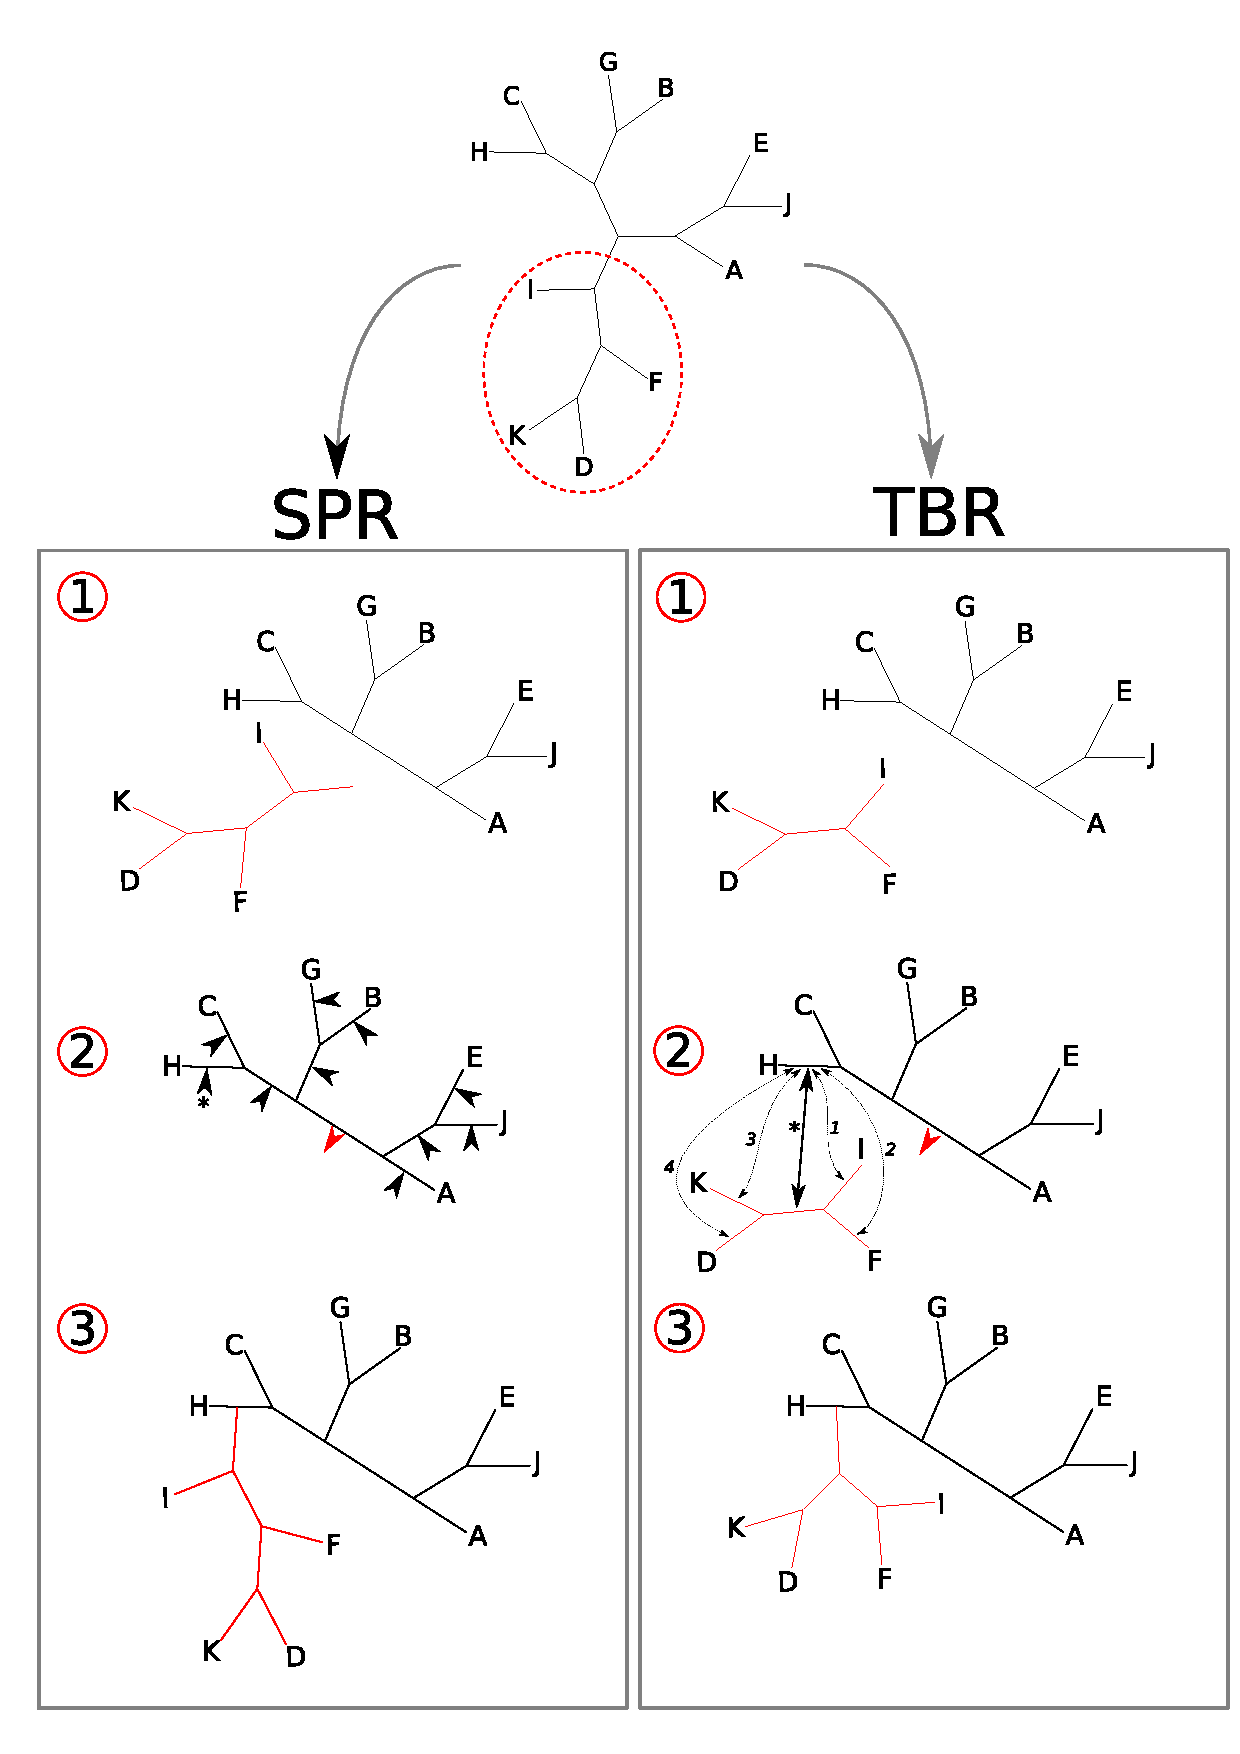
\includegraphics[width=0.8\textwidth]{Figure/FelsensteinFigure.pdf}
\caption{\scriptsize{SPR and TBR description. Modified from \cite{felsenstein2004inferring}, Figure 4.5 and 4.6. \textbf{SPR-1:} blabla; \textbf{SPR-2:} blabla; \textbf{SPR-3:}blabla; \textbf{TBR-1:} blabla; \textbf{TBR-2:} blabla (note that when the sub-tree is reroot on position \textit{1}, the rearrangement is equivalent to a SPR); \textbf{TBR-3:}blabla.}}
\label{Figure_Felsenstein}
\end{figure}


\section{Other}
NNI
tree-fusing
Genetic algorithms
Tree windows and sectorial search
Coalescent with Recombination

\section{Improved algorithm}

\subsection{Neighbour Rule}
Neighbour Rule described \citep[in other words;][]{allen2001subtree}.

\subsection{SPR as TRB (Subtree Rerooting and Branching)}

\section{Conclusion}

This way is not different than the classic SPR/TBR but it's a better implementation.

\section{Data availability and reproducibility}
%TG: Probably some link to morphy


\section{Acknowledgments}
European Research Council under the European Union’s Seventh Framework Programme (FP/2007–2013)/ERC Grant Agreement number 311092.


\bibliographystyle{sysbio}
\bibliography{References}

\end{document}



% For a tree ((A,B),C,(D,E));

% 1 - Clip A and rebranch everywhere:
% ((A,B),C,(D,E));
% (B,(C,A),(D,E));
% (B,C,((A,D),E));
% (B,C,(A,(A,E)));
% That’s 4 trees including the original one!
% If reach 0 trees, go to 4.

% 2 - Clip (A,B) and rebranch everywhere:
% blablabal…
% 3 trees
% If reach 0 trees, go to 4.

% 3- Clip ((A,B),C) and rebranch everywhere:
% blabalbalba…
% 0 trees
% If reach 0 trees, go to 4.

% 4 - Clip !A, rebranch everywhere BUT not to the neighbour branches.
% blablalba.
% 2 trees * (number of tips - 1)  = 8 // The -1 is A
% If reach 0 trees, go to 6.

% 5 - Clip all dichotomies !(A.B), rebranch everywhere BUT not to the neighbour branches/
% blabalbal…
% 0 trees.

% If reach 0 trees, go to 6.
% 6 - Stop

% That’s all folks! Using this algorithm you get… 30 trees!
% Okay, I think it look nicer on paper (I’ll show you tomorrow morning) but it works totally! One only detail that we can improve (and I suspect that’s what PAUP is fucking up) is that step 2, (as step 1) re-includes the original tree (hard to show on unrooted onewicks but obvious on paper). We can reach our 29 trees by removing that one!